\cia\vspace{-2cm}
\section{Absolute normalization of the cross section}
\subsection{Accumulated Faraday Cup}
During the data acquisition the beam charge impinging on the target was saved in the data 
stream as accumulated charge, corrected for live-time by a Faraday cup reading located in the beam dump.
This is a particular event in the data stream called {\it scaler} event.
It consist of a counter whose output $F_{CUP}$ is proportional to the accumulated charge by the relation:
$$
Q^i (Coulombs) = \Dfrac{F^i_{CUP}}{9264.0 \cdot 10^9}
$$
The $F_{CUP}$ reading is performed approximately every 10 second, and it is labelled with an event number
$i$.

Since one run was typically divided into several files, it is possible that the last
Faraday cup reading does not correspond to the accumulated charge for the run because
of corrupted i/o (for example one file can be lost). This is a rare occurence
but must be taken into account. 

To calculate the Faraday cup for a run the difference between
one scaler reading and the next is calculated and saved
$$
\Delta F_{CUP} = F_{CUP}^{i'} - F_{CUP}^i
$$ 
only when $i' = i+1$ (otherwise $\Delta F_{CUP}=0$ ). The $\Delta F_{CUP}$ obtained is then summed 
over all scaler events. \\

For the e1-6 running period the total Faraday cup reading was $F_{CUP} = 2.06816e+11$ for a total charge
$$
Q = 0.022325\;\;{\rm Coulomb}
$$
Assuming a constant current $I=7\,nA$ this gives a running time $t=Q/c\sim 3.2 M {\rm sec} \sim 37$ days.
The number of accelerated electrons was
$$
n_e = Q/e = 1.3934 \cdot 10^{17}
$$
where $e$ is the electron charge.
The number of target nuclei per $cm^2$ can be calculated with the formula:
$$
n_P = \Dfrac{L\,\rho\,N_A}{a.m.u.}
$$
where $L=5$ cm is the length of the target, $\rho=0.0708$ g/cm$^3$ is the density of $H_2$ at $20$K,
$A= 6.022\cdot10^{23}$ mol$^{-1}$ is the Avogadro number and $a.m.u. = 1.00794$ g/mol is the atomic mass unit 
of the hydrogen.
This gives
$$
n_P = 2.115\cdot 10^{23} {\rm cm^{-2}}
$$
So the integrated luminosity for the e1-6 period was
$$
L_{int} = 2.95\cdot 10^{40} {\rm cm^{-2}}
$$

\subsection{Check of normalization}
To estimate the quality of the normalization a comparison of the data with
previous measured and theoretical total c.m. cross sections at lower $Q^2$ is performed.
Equation (\ref{eqno:diffcross}) can be  integrated
over d$\Omega ^*$ to find out that the total cross section is proportional to
$|M_{1+}|^2$:

\begin{equation}
\sigma_{TOT}^{\pi^0} = 8\pi\, \, \Dfrac{2W}{W^2-m_P^2} \,\, |M_{1+}|^2
\end{equation}
so that $|M_{1+}|^2$ can be used as normalization check.

\F{fig:MM} shows the $|M_{1+}|^2$ at the peak of the $\Delta$ as a function of $Q^2$.
The data from \cite{bib:frolov} and the MAID and DMT predictions are also shown.
Good agreement is found with previous results and the two models.

\begin{figure}[h]
 \begin{center}
  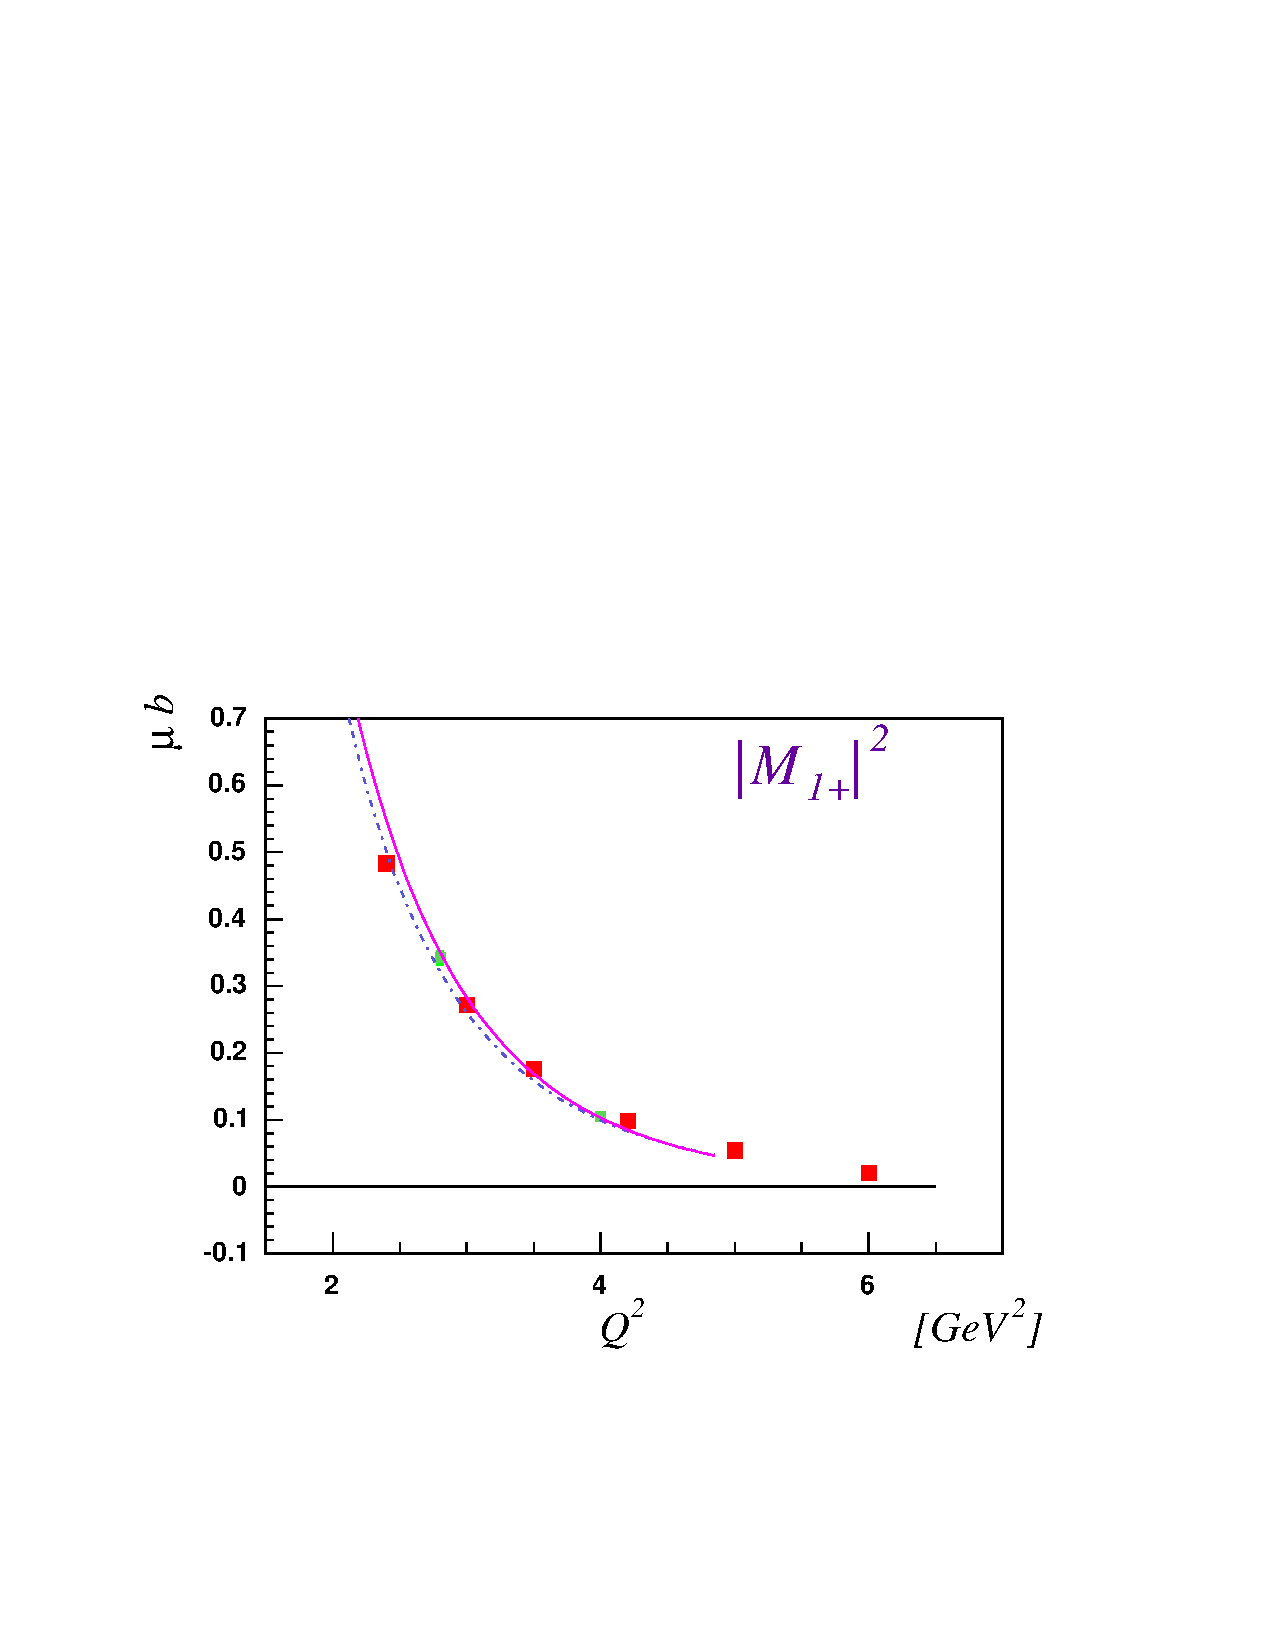
\includegraphics[width=14cm, bb=40 100 520 460]{analysis/img/MM}
  \caption[$|M_{1+}|^2$ at the peak of the $\Delta$ as a function of $Q^2$]
          { $|M_{1+}|^2$ at the peak of the $\Delta$ as a function of $Q^2$.
	             The green points come from \cite{bib:frolov}. The solid line is due to MAID, 
		     the dashed line is due to DMT.}
 \label{fig:MM}
  \end{center} 
\end{figure} 





















